% Copyright Aidan Randle-Conde 2007-2014
% http://www.aidansean.com/phd_notes
% Anyone is free to download, redistribute, edit and use these notes and the source tex files with the following restrictions:
% This 
%  This message is included in the tex source files.
%  Aidan Randle-Conde is credited as the author.
%  Images are correctly credited to their respective authors, as outlined in the references.
%  No part of these notes may be used for commercial purposes.

\chapter{Spinless \texorpdfstring{$\lowercase{e}^- \mu^-$}{EMu} scattering}

\section{Electrodynamics of spinless particles}

\begin{figure}[!htb]
  \begin{center}
    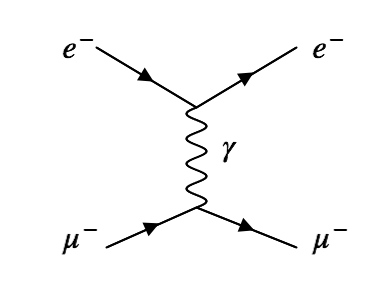
\includegraphics[width=0.5\textwidth]{images/web_feynman/image_20.png}
    \caption[Spinless $e-\mu$ scattering]{Feynman diagram showing spinless $e-\mu$ scattering.}
    \label{fig:ch7_EMuToEMu}
  \end{center}
\end{figure}

Consider spinless electrons scattering off spinless muons, as shown in figure \ref{fig:ch7_EMuToEMu}.  Starting with the Klein-Gordon equation and including the electromagnetic interaction will lead to a simple model of scattering.  In electrodynamics the motion of a particle of charge $-\e$ in an electromagnetic potential $A^{\mu} (= (A^0,\ul{A}))$ is obtained by the substitution:

\begin{eqnarray*}
  p^{\mu} & \to & p^{\mu} + \e A^{\mu} \\
  \textrm{So } p_{\mu}p^{\mu} = m^2 & \to & \left(p_{\mu} + \e A_{\mu} \right)\left(p^{\mu} + \e A^{\mu}\right) = m^2
\end{eqnarray*}

In quantum mechanics this is:

\begin{eqnarray*}
  \left(i\partial_{\mu} + \e A_{\mu}\right)\left(i\partial^{\mu} + \e A^{\mu}\right)\phi & = & m^2 \phi \\
  -\partial_{\mu}\partial^{\mu}\phi + i\e \partial_{\mu}A^{\mu}\phi + i\e A_{\mu}\partial^{\mu}\phi + \e^2A_{\mu}A^{\mu}\phi & = & m^2\phi \\
  \Rightarrow \partial_{\mu}\partial^{\mu} + m^2\partial & = & ie\partial_{\mu}A^{\mu}\phi + i\e A_{\mu}\partial^{\mu}\phi + \e^2A_{\mu}A^{\mu}\phi \\
  & = & -V\phi
\end{eqnarray*}

where $V$ is the electromagnetic perturbation and the minus sign is required to that there is the same relateive sign to the $p^2/2m$ term in the Schroedinger equation.

The transition amplitude is:

\begin{eqnarray*}
  T_{fi} & = & -i\int\mathrm{d}^4x\phi^{\star}_f(x)V(x)\phi_i(x) \\
         & = & -i\int\mathrm{d}^4x\phi^{\star}_f(x)(-i\e)(\partial_{\mu}A^{\mu} + A_{\mu}\partial^{\mu})\phi_2(x)
\end{eqnarray*}
where the second order term is neglected.

Transforming the first term so that the derivative acts on $\phi^{\star}_f$:

\begin{eqnarray*}
  T_{fi} & = & \int \phi^{\star}_f \partial_{\mu}\left(A^{\mu}\phi_2\right)\mathrm{d}^4x + \cdots \\
  I & = & \int \phi^{\star}_f\partial_{\mu}\left(A^{\mu}\phi_2\right)\mathrm{d}^4x \\
  \int u\frac{\mathrm{d}v}{\mathrm{d}x}\mathrm{d}x & = & uv - \int v \frac{\mathrm{d}u}{\mathrm{d}x}\mathrm{d}x \\
  \textrm{So let } u & = & \phi^{\star}_f \\
  \frac{\mathrm{d}v}{\mathrm{d}x} & = & \partial_{\mu}\left(A^{\mu}\phi_i\right) \\
  \textrm{So } I & = & \Bigg[ \phi^{\star}_fA^{\mu}\phi_i\Bigg]_{-\infty}^{\infty} - \int\mathrm{d}^4x\left(\partial_{\mu}\phi^{\star}_f\right)A^{\mu}\phi_i \\
  \textrm{So }T_{fi} & = & -\e\int\mathrm{d}^4x\left(\phi^{\star}_fA_{\mu}\partial^{\mu}\phi_i - \partial_{\mu}\phi^{\star}_fA^{\mu}\phi_i\right) \\
  & = & -i\int\mathrm{d}^4xA^{\mu}j^{fi}_{\mu} \\
  \textrm{where } j^{fi}_{\mu} & = & -ie\left(\phi^{\star}_f\left(\partial_{\mu}\phi_i\right) - \left(\partial_{\mu}\phi^{\star}_f\right)\phi_i\right)
\end{eqnarray*}

At the top vertex the particle $A$ is described by:

\[
  \phi_A(x) = N_A\e^{-ip_Ax}
\]

Similarly, particle $C$ is described by:

\begin{eqnarray*}
  \phi_C(x) & = & N_C\e^{-ip_Cx} \\
  \Rightarrow j^{CA}_{\mu}(x) & = & -i\e\Big[N^{\star}_C\e^{ip_Cx}N_A\e^{-ip_Ax}\left(-ip_A\right)_{\mu} - N^{\star}_C \e^{ip_Cx}\left(ip_C\right)_{\mu}N_A\e^{-ip_Ax}\Big] \\
  & = & -i\e N^{\star}_CN_A\e^{i\left(p_C-p_A\right)x}\left(-ip_A-ip_C\right)_{\mu} \\
  & = & -\e N^{\star}_CN_A\left(p_A+p_C\right)_{\mu}\e^{i\left(p_C-p_A\right)x}
\end{eqnarray*}

and similarly for $j^{BD}_{\mu}$

For $A^{\mu}$, using Maxwell's equations:

\begin{equation}
  \Box^2A^{\mu}(x) = j^{\mu}(x) \label{eq:boxaj}
\end{equation}

The solution is found by inspection and the field $A^{\mu}$ arises because of the field from the current at the lower vertex:

\[
  j^{\mu}_{DB} = -\e N^{\star}_DN_B\left(p_B + p_D\right)^{\mu}\e^{i\left(p_D-p_B\right)x}
\]

By inspection the substitution

\[
  A^{\mu} = \frac{-g^{\mu\nu}j^{DB}_{\nu}}{q^2}
\]

satisfies (\ref{eq:boxaj}) where $q = p_D - p_B$.

Substituting this into (\ref{eq:boxaj}) gives:

\begin{eqnarray*}
  \partial_{\mu}\partial^{\mu}\left(\frac{-1}{q^2}\right)j^{\mu}_{DB} & = & \frac{-1}{q^2}j^{\mu}_{DB}\Big[-i\left(p_D-p_B\right)\Big]^2 \\
  & = & \frac{1}{q^2}j^{\mu}_{DB}q^2
\end{eqnarray*}

So the expression for $A^{\mu}$ satisfies (\ref{eq:boxaj}).

\begin{eqnarray*}
  T_{fi} & = & -i\int\mathrm{d}^4xj^{CA}_{\mu}(x)A^{\mu} \\
  & = & -i\int\mathrm{d}^4x\left(-\e\right)N^{\star}_CN_A\left(p_A + p_C\right)_{\mu}\e^{i\left(p_C-p_A\right)x}\left(\frac{-1}{q^2}\right)\left(-\e\right)N^{\star}_DN_B\left(p_B + p_D\right)^{\mu}\e^{i\left(p_D-p_B\right)x} \\
  & = & \frac{i\e^2}{q^2}\int N^{\star}_CN_AN^{\star}_DN_B\left(p_A+p_C\right)_{\mu}\left(p_D+p_B\right)^{\mu}\e^{i\left(p_C+p_D-p_A-p_B\right)x}\mathrm{d}^4x
\end{eqnarray*}

\section{Definition of the cross section}

The cross section is imagined to take place in an intercation volume $V$ and the normalisation is such that there are $2E$ particles of each kind ($A$, $B$, $C$, $D$) in this volume.

\begin{eqnarray*}
  \textrm{If }\phi_A & = & N_A\e^{ip_Ax} \\
  \textrm{then }\int\rho\mathrm{d}^3r & = & \int 2E\phi^{\star}_A\phi_A\mathrm{d}^3r \\
  & = & 2EN^{\star}_AN_AV \\
  & = & 2E \\
  \textrm{where }N_A & = & \frac{1}{\sqrt{V}}
\end{eqnarray*}

$T_{fi}$ is the amplitude of transmission from an initial state $i$ to a final state $f$.  The number of transitions per unit time per unit volume, $W_{fi}$ is given by:

\[
  W_{fi} = \frac{T_{fi}T^{\star}_{fi}}{\textrm{Unit time and volume}}
\]

The cross section is then given by:

\begin{eqnarray*}
  \sigma & = & W_{fi}\left(\frac{\textrm{number of final states}}{\textrm{initial flux}}\right) \\
  T_{fi}T^{\star}_{fi} & = & \frac{\e^4}{q^4}\int\int \frac{1}{V^4}\Big[\left(p_A+p_C\right)_{\mu}\left(p_B+p_D\right)^{\mu}\Big]^2 \e^{i\left(p_C+p_D-p_A-p_B\right)x}\e^{-i\left(p_C+p_D-p_A-p_B\right)x'}\mathrm{d}^4x\mathrm{d}^4x' \\
  W_{fi} & = & \frac{\e^4}{q^4V^4}\Big[\left(p_A+p_C\right)_{\mu}\left(p_B+p_D\right)^{\mu}\Big]^2\delta^4\left(p_C+p_D-p_A-p_B\right)\frac{2\pi^4TV}{TV} \\
  & = & \frac{\e^4}{q^4V^4}\Big[\left(p_A+p_C\right)_{\mu}\left(p_B+p_D\right)^{\mu}\Big]^2\delta^4\left(p_C+p_D-p_A-p_B\right)2\pi^4 \\
  & = & \frac{\e^4}{q^4}\frac{2\pi^4}{V^4}\Big[\left(p_A+p_C\right)_{\mu}\left(p_B+p_D\right)^{\mu}\Big]^2\delta^4\left(p_C+p_D-p_A-p_B\right)
\end{eqnarray*}

Consider the number of final states.  Each particle in the final state has a three momentum between $\ul{p}_C$ and $\ul{p}_C + \mathrm{d}^3\ul{p}_C$, and $\ul{p}_D$ and $\ul{p}_D + \mathrm{d}^3\ul{p}_D$ and energies between $E_C$ and $E_C + \mathrm{d}E_C$, and $E_D$ and $E_D + \mathrm{d}E_D$.  The number of final states per unit volume is determined by constraints imposed by the $\delta$ function.  These particles are imagined to be travelling in waves, which enter and leave the interaction volume, $V$.  The propagator particle only exists within the interaction volume, so it must have the wavefunction of a particle in an infinite square well, leading to quantisation of the transfer momentum.

Suppose the entrance is at $x = 0$ and the exit is as $x = L_x$, then:

\[
  p_xL_x = 2\pi n_x \quad n_x \in N
\]

and similarly for $y$ and $z$.

The momentum separation, $\Delta p_x$ is given by:

\begin{eqnarray*}
  \left(p_x + \Delta p_x\right) L_x & = & 2\pi\left(n_x + 1\right) \\
  \Rightarrow \Delta p_x & = & \frac{2\pi}{L_x}
\end{eqnarray*}

Therefore the number of final states is:

\begin{eqnarray*}
  N_f & = & \frac{\mathrm{d}p_x}{2\pi}\frac{\mathrm{d}p_y}{2\pi}\frac{\mathrm{d}p_z}{2\pi}L_xL_yL_z \\
  & = & \frac{V}{\left(2\pi\right)^3}\mathrm{d}^3p
\end{eqnarray*}

There are $2E$ particles in $V$, so the normalised number of states is:

\[
  N_f = \frac{V}{\left(2\pi\right)^3}2E\mathrm{d}^3p
\]

Summing over states in $C$ and $D$:

\[
  N^{CD}_f = \frac{V\mathrm{d}^3p_C}{\left(2\pi\right)^3E_C}\frac{V\mathrm{d}^3p_D}{\left(2\pi\right)^2E_D}
\]

The flux factor is $\rho_A\rho_B u_{AB}$ where $\rho_i$ is the desnity of particles in $V$ and $u_{AB}$ is the relative velocity of particles $A$ and $B$.

\begin{eqnarray*}
  u_{AB} & = & u_A - u_B \\
  \Rightarrow flux & = & \frac{2E_A}{V}\frac{2E_B}{V}u_{AB} \\
  & = & \frac{2E_A}{V}\frac{2E_B}{V}\left(\frac{p_A}{E_A}-\frac{P_B}{E_B}\right) \\
  & = & \frac{4E_AE_B}{V^2}\left(\frac{p_AE_B-E_Ap_B}{E_AE_B}\right) \\
  & = & \frac{4}{V^2}\left(p_AE_B -p_BE_A\right)
\end{eqnarray*}

In the centre of mass system $p_A = p_B$, so:

\begin{eqnarray*}
  flux & = & \frac{4}{V^2}p_A\left(E_A + E_B\right) \\
  & = & \frac{4}{V^2}p_A\sqrt{s}
\end{eqnarray*}

Combining all the terms into the cross section formula gives:

\begin{eqnarray*}
  \mathrm{d}\sigma & = & \frac{\e^4}{q^4}\frac{\left(2\pi\right)^4}{V^4}\Big[\left(p_A+p_C\right)_{\mu}\left(p_B+p_D\right)^{\mu}\Big]^2\delta^4\left(p_C+p_D-p_A-p_B\right) \\ 
  & & \times\frac{V\mathrm{d}^3p_C}{2E_C}\frac{1}{\left(2\pi\right)^3}\frac{V\mathrm{d}^3p_D}{2E_D}\frac{1}{\left(2\pi\right)^3}\frac{V^2}{4p_A\sqrt{s}}
\end{eqnarray*}

The Lorentz invariant phase space, $\mathrm{d}Q$ is given by:

\[
  \mathrm{d}Q = \frac{V}{2E_C}\frac{\mathrm{d}^3p_C}{\left(2\pi\right)^3}\frac{V}{2E_D}\frac{\mathrm{d}^3p_D}{\left(2\pi\right)^3}\left(2\pi\right)^4\delta\left(p_C+P_D-p_A-p_B\right)
\]

In the centre of mass system:

\[
  \mathrm{d}Q  = \left(2\pi\right)^4\delta\left(\sqrt{s}-\left(E_C+E_D\right)\right)\delta^3\left(p_C+p_D\right)\frac{\mathrm{d}^3p_C}{2E_C}\frac{1}{\left(2\pi\right)^3}\frac{\mathrm{d}^3p_D}{2E_D}\frac{1}{\left(2\pi\right)^3}V^2
\]

The degree of the differential can be reduced by integrating over $\mathrm{d}^3p_D$:

\[
  \mathrm{d}Q = \left(2\pi\right)^4\delta\left(\sqrt{s}-\left(E_C+E_D\right)\right)\frac{\mathrm{d}^3p_C}{2E\left(2\pi\right)^3}\frac{1}{2E_D\left(2\pi\right)^3}V^2
\]

The integration over $\mathrm{d}^3p_C$, using the angle $\theta$ as defined in figure \ref{fig:ch7_EMuToEMuScatterAngle}, is given by:

\begin{eqnarray*}
  \int\mathrm{d}^3p_C & = & \int 2\pi p_C\sin\theta p_C\mathrm{d}\theta\mathrm{d}p_C \\
  & = & \int p_C^2\mathrm{d}p_C \left(2\pi\sin\theta\mathrm{d}\theta\right) \\
  & = & \int p_C^2 \mathrm{d}p_C \mathrm{d}\Omega \\
  \textrm{so } \mathrm{d}Q & = & \frac{V^2}{\left(4\pi\right)^2} \delta\left(\sqrt{s}-\left(E_C + E_D\right)\right)\frac{1}{4E_CE_D}p_C^2 \mathrm{d}p_C\mathrm{d}\Omega
\end{eqnarray*}

\begin{figure}[!htb]
  \begin{center}
    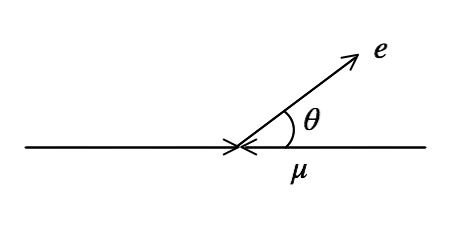
\includegraphics[width=0.75\textwidth]{images/web_feynman/image_21.png}
    \caption[Angle between $e$ and $\mu$ in $e-\mu$ scattering]{Definition of the angle between the electron and muon in the scattering process, $\theta$.}
    \label{fig:ch7_EMuToEMuScatterAngle}
  \end{center}
\end{figure}

In the centre of mass system:

\begin{eqnarray*}
  \sqrt{s} & = & \left(E_D + E_D\right) \\
  & = & \sqrt{p_C^2 + m_C^2} + \sqrt{p_D^2 + m_D^2} \\
  & = & \sqrt{p_C^2 + m_C^2} + \sqrt{p_C^2 + m_D^2} \\
  \Rightarrow \mathrm{d}\sqrt{s} & = & \frac{2p_C\mathrm{d}p_C}{2\sqrt{p_C^2 + m_C^2}} + \frac{2p_C\mathrm{d}p_C}{2\sqrt{p_C^2 + m_D^2}} \\
  & = & p_C \mathrm{d}p_C\left(\frac{1}{\sqrt{p_C^2 + m_C^2}} + \frac{1}{\sqrt{p_D^2 + m_D^2}}\right) \\
  & = & p_C\mathrm{d}p_C\left(\frac{1}{E_C} + \frac{1}{E_D}\right) \\
  & = & p_C\left(\frac{E_D + E_C}{E_DE_C}\right)\mathrm{d}p_C \\
  & = & \frac{p_C\sqrt{s}\mathrm{d}p_C}{E_CE_D} \\
  \Rightarrow \mathrm{d}Q & = & \frac{V^2}{4\pi^2}\delta(\sqrt{s}-\left(E_C + E_D\right))\frac{1}{4}\mathrm{d}\Omega\frac{1}{E_CE_D}p_C^2\mathrm{d}p_C \\
  & = & \frac{V^2}{4\pi^2}\delta\left(\sqrt{s}-\left(E_C+E_D\right)\right)\frac{1}{4}\mathrm{d}\Omega\frac{p_C}{\sqrt{s}}\sqrt{s} \\
  & = & \frac{V^2}{16\pi^2}\mathrm{d}\Omega\frac{\mathrm{d}p_C}{\sqrt{s}} \\
  \Rightarrow \mathrm{d}\sigma & = & \frac{\e^4}{q^4}\frac{1}{V^4}\Big[\left(p_A + p_C\right)_{\mu}\left(p_B + p_D\right)^{\mu}\Big]^2\mathrm{d}Q\frac{V^2}{4p_A\sqrt{s}} \\
  & = & \frac{\e^4}{q^4}\frac{1}{V^4}\Big[\left(p_A + p_C\right)_{\mu}\left(p_B + p_D\right)^{\mu}\Big]\frac{V^2}{4p_A\sqrt{s}}\frac{V^2}{16\pi^2}\mathrm{d}\Omega\frac{p_C}{\sqrt{s}} \\
  \frac{\mathrm{d}\sigma}{\mathrm{d}\Omega} & = & \frac{\e^4}{q^4}\frac{1}{64\pi^2}\frac{\Big[\left(p_A+p_C\right)_{\mu}\left(p_B+p_D\right)^{\mu}\Big]^2p_C}{p_As}
\end{eqnarray*}

The number of final states divided by the flux factor in two body processes is used in many calculations and is:

\[
  \frac{1}{64\pi^2s}\frac{p_C}{p_A}
\]

Consider the cross-section for the massless limit, $m_i \to 0$ or $E_i \gg m_i$, as shown in figure \ref{fig:ch7_particleScattering}, and the definition of $\theta$ shown in figure \ref{fig:ch7_genericScatterAngle}.

\begin{figure}[!htb]
  \begin{center}
    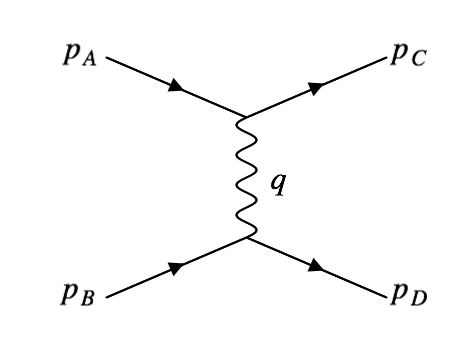
\includegraphics[width=0.5\textwidth]{images/web_feynman/image_22.png}
    \caption[Scattering of massless particles]{Scattering of massless particles.  The momenta are related by $p_A=p_C+q$ and $p_D=p_B+q$.}
    \label{fig:ch7_particleScattering}
  \end{center}
\end{figure}

\begin{figure}[!htb]
  \begin{center}
    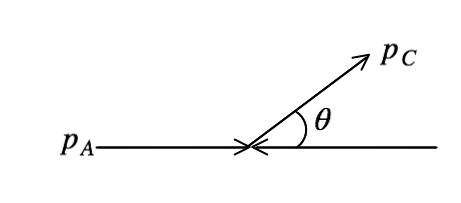
\includegraphics[width=0.75\textwidth]{images/web_feynman/image_23.png}
    \caption[Definition of $\theta$ for a scattering of massless particles]{Definition of $\theta$ for a generic scattering process.}
    \label{fig:ch7_genericScatterAngle}
  \end{center}
\end{figure}

\begin{eqnarray*}
  q^2 & = & \left(p_A - p_C\right)^2 \\
  & = & \left(E_A - E_C,\ul{p}_A - \ul{p}_C\right)^2 \\
  \textrm{For } m \to 0 \quad |\ul{p}_A| & \simeq & E_A \textrm{ etc} \\
  \Rightarrow q^2 & = & \left(E_A - E_C\right)^2 - \left(\ul{p}_A - \ul{p}_C\right)^2 \\
  & = & E_A^2 + E_C^2 - 2E_AE_C - \left(\ul{p}_A - \ul{p}_C\right)^2 \\
  & = & -2E_AE_C + 2\ul{p}_A\cdot\ul{p}_C \\
  & = & -2E_AE_C \left(1 - \cos \theta\right) \\
  \textrm{So } q^4 & = & 4E_A^2E_C^2\left(1 - \cos\theta\right)^2 \\
  \Big[\left(p_A + p_C\right)_{\mu}\left(p_B + p_D\right)^{\mu}\Big]^2 & = & \Big[p_A\cdot p_B + p_A\cdot p_D +p_B\cdot p_C + p_C\cdot p_D \Big]^2 \\
  \textrm{Using } p_A & = & \left(|\ul{p}|,\ul{p} \right) \\
  p_B & = & \left(|\ul{p}|,-\ul{p} \right) \\
  p_C & = & \left(|\ul{p}|,\ul{p}' \right) \\
  p_D & = & \left(|\ul{p}|,-\ul{p}' \right) \\
  \textrm{With } |\ul{p}| & = & |\ul{p}'| \\
  \Rightarrow \Big[\left(p_A + p_C\right)_{\mu}\left(p_B + p_D\right)^{\mu}\Big]^2 & = & \left(6p^2 + 2p^2\cos\theta\right)^2 \\
  \Rightarrow \left(\frac{\mathrm{d}\sigma}{\mathrm{d}\Omega}\right)_{e\mu} & = & \frac{\e^4}{64\pi^4s}\left(\frac{3 + \cos\theta}{1 - \cos\theta}\right)^2
\end{eqnarray*}

\subsection{Note on decay}

Consider the number of states per flux factor for the decay $A \to B \quad C$.

The number of states is as before:

\[
  \frac{1}{16\pi^2}\frac{p_CV^2}{m_A}\mathrm{d}\Omega
\]

Due to the choice of normalisation there are $2E_m$ particles per state in the centre of mass frame in a volume $V$:

\[
  \rho = \frac{2m_A}{V}
\]

The flux factor is:

\begin{eqnarray*}
  F & = & \frac{1}{16\pi^2}\frac{p_CV^2}{m_A}\mathrm{d}\Omega\frac{V}{2m_A} \\
    & = & \frac{1}{32\pi^2}\frac{p_C}{m_A^2}V^3\mathrm{d}\Omega
\end{eqnarray*}

The decay rate is:

\[
  \frac{\mathrm{d}\Gamma}{\mathrm{d}\Omega} = |T_{fi}|^2\frac{1}{32\pi^2}\frac{p_C}{m_A^2}V^3\mathrm{d}\Omega
\]


This factor is universal for decays if the decay is istropic:

\begin{eqnarray*}
  \mathrm{d}\Omega & \to & 4\pi \\
  \mathrm{d}\Gamma & \to & \Gamma
\end{eqnarray*}

For the decay of $A$:

\[
  \frac{\mathrm{d}N_A}{\mathrm{d}t} = \Gamma N_A
\]

ie $N_A(t) = N_A(0)e^{-\Gamma t}$ and $\Gamma^{-1}$ is the mean lifetime.
